\chapter{Browsing with Tree}\label{chap:browsing}

Before we open up a document to study, we have to know how to find the text first. There are two ways to do this. First, we can approach a text by a hierarchical tree structure of each collection using \emph{TOC Tree} window. And second, we can find a specific text by a given criterion using \emph{Document Finder} window. This chapter will talk about the former. For the latter, see Chapter \ref{chap:finder}.

You can use TOC\,Tree by its tab in the main window, or you can open a new window by {\faSix \symbol{"F802}} button or menu Reader > {\faSix \symbol{"F802}} TOC\ Tree. Once you see the tree, you can expand its branches by clicking a node. Figure \ref{fig:toctree-expanded} shows the selection of the first book of Dīghanikāya in the collection of CST Restructured.

\dothis{You can see the filename of each document by toggle {\faSix \symbol{"F02C}} button on the window's tool bar.\\
\hspace{5mm} You can see information of the collection selected by clicking {\faSix \symbol{"F129}} button.
}

At the level of file as shown by the icon, the document can be opened with a context menu provided. Behind the name of a document, its reference according to the scheme of the corpus is shown in parentheses. For example, in the picture \emph{d1} (or D1) is used for Sīlakkhandhavagga of Dīghanikāya in the CSTR collection.

\begin{figure}[!hbt]
\centering
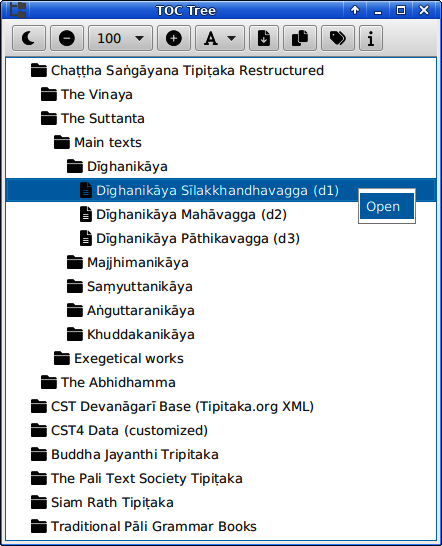
\includegraphics[width=0.8\linewidth]{images/toctree-expanded.png}\\
\caption{TOC Tree expanded to file level}
\label{fig:toctree-expanded}
\end{figure}

Please note that the tree structure of each Tipiṭaka collection follows the same grouping scheme. That is to say, the division into three baskets (Vinaya, Suttanta, Abhidhamma) is primary and the division of main (mūla) and exegetical works (aṭṭhakathā, ṭīkā) is secondary. Some collections have an extra group as well.

